% Options for packages loaded elsewhere
\PassOptionsToPackage{unicode}{hyperref}
\PassOptionsToPackage{hyphens}{url}
%
\documentclass[
  12pt,
]{article}
\usepackage{lmodern}
\usepackage{amssymb,amsmath}
\usepackage{ifxetex,ifluatex}
\ifnum 0\ifxetex 1\fi\ifluatex 1\fi=0 % if pdftex
  \usepackage[T1]{fontenc}
  \usepackage[utf8]{inputenc}
  \usepackage{textcomp} % provide euro and other symbols
\else % if luatex or xetex
  \usepackage{unicode-math}
  \defaultfontfeatures{Scale=MatchLowercase}
  \defaultfontfeatures[\rmfamily]{Ligatures=TeX,Scale=1}
\fi
% Use upquote if available, for straight quotes in verbatim environments
\IfFileExists{upquote.sty}{\usepackage{upquote}}{}
\IfFileExists{microtype.sty}{% use microtype if available
  \usepackage[]{microtype}
  \UseMicrotypeSet[protrusion]{basicmath} % disable protrusion for tt fonts
}{}
\makeatletter
\@ifundefined{KOMAClassName}{% if non-KOMA class
  \IfFileExists{parskip.sty}{%
    \usepackage{parskip}
  }{% else
    \setlength{\parindent}{0pt}
    \setlength{\parskip}{6pt plus 2pt minus 1pt}}
}{% if KOMA class
  \KOMAoptions{parskip=half}}
\makeatother
\usepackage{xcolor}
\IfFileExists{xurl.sty}{\usepackage{xurl}}{} % add URL line breaks if available
\IfFileExists{bookmark.sty}{\usepackage{bookmark}}{\usepackage{hyperref}}
\hypersetup{
  pdftitle={LOND Summary of Mediators GTExV8},
  pdfauthor={Jarred Kvamme},
  hidelinks,
  pdfcreator={LaTeX via pandoc}}
\urlstyle{same} % disable monospaced font for URLs
\usepackage[margin=1in]{geometry}
\usepackage{longtable,booktabs}
% Correct order of tables after \paragraph or \subparagraph
\usepackage{etoolbox}
\makeatletter
\patchcmd\longtable{\par}{\if@noskipsec\mbox{}\fi\par}{}{}
\makeatother
% Allow footnotes in longtable head/foot
\IfFileExists{footnotehyper.sty}{\usepackage{footnotehyper}}{\usepackage{footnote}}
\makesavenoteenv{longtable}
\usepackage{graphicx,grffile}
\makeatletter
\def\maxwidth{\ifdim\Gin@nat@width>\linewidth\linewidth\else\Gin@nat@width\fi}
\def\maxheight{\ifdim\Gin@nat@height>\textheight\textheight\else\Gin@nat@height\fi}
\makeatother
% Scale images if necessary, so that they will not overflow the page
% margins by default, and it is still possible to overwrite the defaults
% using explicit options in \includegraphics[width, height, ...]{}
\setkeys{Gin}{width=\maxwidth,height=\maxheight,keepaspectratio}
% Set default figure placement to htbp
\makeatletter
\def\fps@figure{htbp}
\makeatother
\setlength{\emergencystretch}{3em} % prevent overfull lines
\providecommand{\tightlist}{%
  \setlength{\itemsep}{0pt}\setlength{\parskip}{0pt}}
\setcounter{secnumdepth}{-\maxdimen} % remove section numbering

\title{LOND Summary of Mediators GTExV8}
\usepackage{etoolbox}
\makeatletter
\providecommand{\subtitle}[1]{% add subtitle to \maketitle
  \apptocmd{\@title}{\par {\large #1 \par}}{}{}
}
\makeatother
\subtitle{Audrey Fu Lab}
\author{Jarred Kvamme}
\date{4/8/2021}

\begin{document}
\maketitle

\begin{longtable}[]{@{}lrr@{}}
\caption{Total number of Cis and Trans genes identified as Mediators
under MRPC-LOND}\tabularnewline
\toprule
& Total.Num.Genes & Percent.Of.Total\tabularnewline
\midrule
\endfirsthead
\toprule
& Total.Num.Genes & Percent.Of.Total\tabularnewline
\midrule
\endhead
Cis Only & 1715 & 0.3977273\tabularnewline
Trans Only & 2506 & 0.5811688\tabularnewline
Both Cis \& Trans & 91 & 0.0211039\tabularnewline
\bottomrule
\end{longtable}

\begin{longtable}[]{@{}lrr@{}}
\caption{Total number of Unqiue Cis and Trans genes identified as
Mediators under MRPC-LOND}\tabularnewline
\toprule
& Total.Unique.Genes & Percent.Of.Total\tabularnewline
\midrule
\endfirsthead
\toprule
& Total.Unique.Genes & Percent.Of.Total\tabularnewline
\midrule
\endhead
Cis Only Unique & 1005 & 0.3356713\tabularnewline
Trans Only Unique & 1898 & 0.6339345\tabularnewline
Both Cis \& Trans & 91 & 0.0303941\tabularnewline
\bottomrule
\end{longtable}

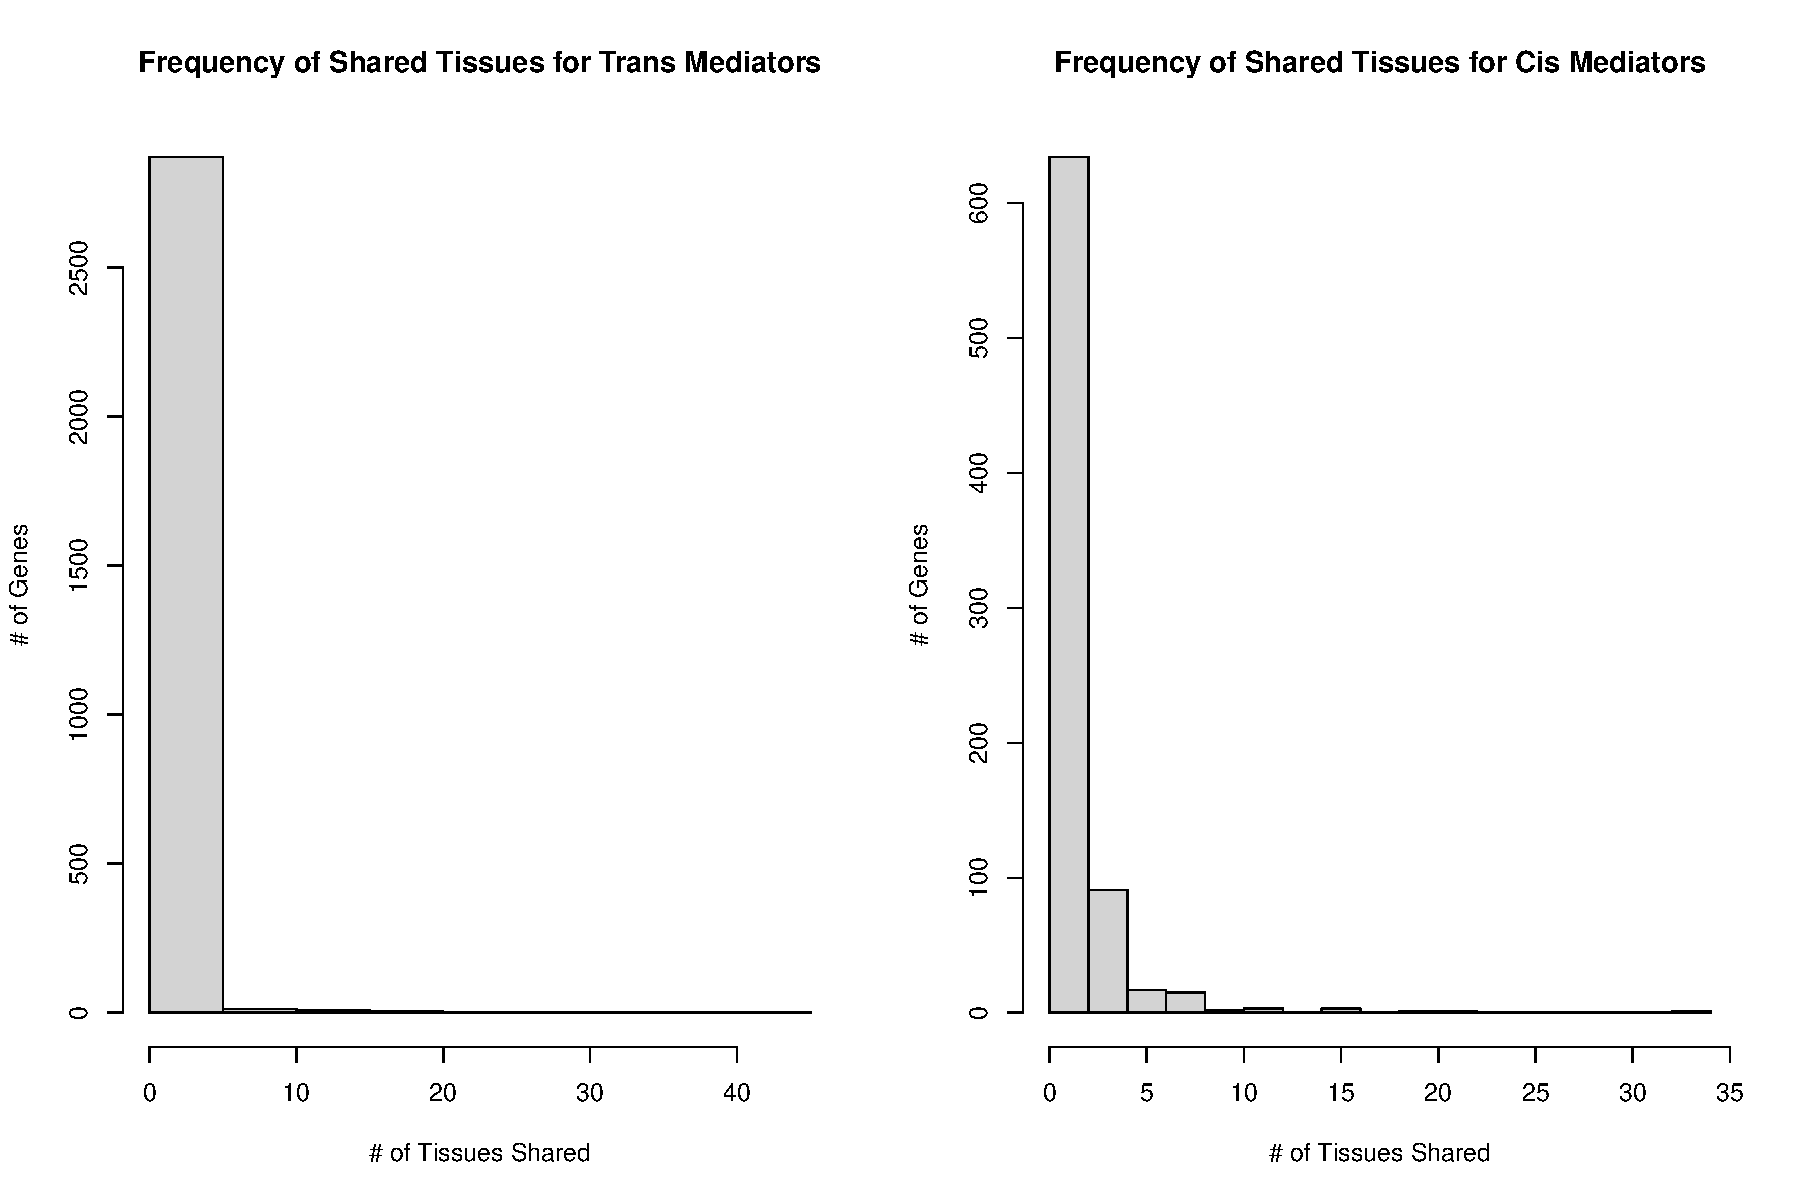
\includegraphics{LOND_Summary_mediator_GTExV8_files/figure-latex/unnamed-chunk-2-1.pdf}

\begin{longtable}[]{@{}rr@{}}
\caption{LOND Trans Mediator Tissue Counts}\tabularnewline
\toprule
Number of Genes & Number of Tissues Shared\tabularnewline
\midrule
\endfirsthead
\toprule
Number of Genes & Number of Tissues Shared\tabularnewline
\midrule
\endhead
1804 & 1\tabularnewline
90 & 2\tabularnewline
17 & 3\tabularnewline
11 & 4\tabularnewline
4 & 5\tabularnewline
2 & 6\tabularnewline
5 & 7\tabularnewline
1 & 8\tabularnewline
2 & 9\tabularnewline
2 & 10\tabularnewline
1 & 11\tabularnewline
2 & 12\tabularnewline
2 & 13\tabularnewline
2 & 14\tabularnewline
3 & 15\tabularnewline
0 & 16\tabularnewline
0 & 17\tabularnewline
1 & 18\tabularnewline
0 & 19\tabularnewline
0 & 20\tabularnewline
0 & 21\tabularnewline
0 & 22\tabularnewline
0 & 23\tabularnewline
0 & 24\tabularnewline
0 & 25\tabularnewline
1 & 26\tabularnewline
0 & 27\tabularnewline
0 & 28\tabularnewline
0 & 29\tabularnewline
0 & 30\tabularnewline
0 & 31\tabularnewline
0 & 32\tabularnewline
0 & 33\tabularnewline
1 & 34\tabularnewline
0 & 35\tabularnewline
1 & 36\tabularnewline
0 & 37\tabularnewline
0 & 38\tabularnewline
0 & 39\tabularnewline
0 & 40\tabularnewline
1 & 41\tabularnewline
0 & 42\tabularnewline
0 & 43\tabularnewline
0 & 44\tabularnewline
0 & 45\tabularnewline
0 & 46\tabularnewline
0 & 47\tabularnewline
0 & 48\tabularnewline
\bottomrule
\end{longtable}

\begin{longtable}[]{@{}rr@{}}
\caption{LOND Cis Mediator Tissue Counts}\tabularnewline
\toprule
Number of Genes & Number of Tissues Shared\tabularnewline
\midrule
\endfirsthead
\toprule
Number of Genes & Number of Tissues Shared\tabularnewline
\midrule
\endhead
792 & 1\tabularnewline
129 & 2\tabularnewline
55 & 3\tabularnewline
31 & 4\tabularnewline
12 & 5\tabularnewline
13 & 6\tabularnewline
8 & 7\tabularnewline
1 & 8\tabularnewline
1 & 9\tabularnewline
3 & 10\tabularnewline
2 & 11\tabularnewline
0 & 12\tabularnewline
2 & 13\tabularnewline
1 & 14\tabularnewline
1 & 15\tabularnewline
0 & 16\tabularnewline
0 & 17\tabularnewline
1 & 18\tabularnewline
0 & 19\tabularnewline
1 & 20\tabularnewline
1 & 21\tabularnewline
0 & 22\tabularnewline
0 & 23\tabularnewline
1 & 24\tabularnewline
1 & 25\tabularnewline
0 & 26\tabularnewline
0 & 27\tabularnewline
0 & 28\tabularnewline
0 & 29\tabularnewline
0 & 30\tabularnewline
0 & 31\tabularnewline
0 & 32\tabularnewline
0 & 33\tabularnewline
0 & 34\tabularnewline
0 & 35\tabularnewline
0 & 36\tabularnewline
0 & 37\tabularnewline
0 & 38\tabularnewline
0 & 39\tabularnewline
0 & 40\tabularnewline
1 & 41\tabularnewline
0 & 42\tabularnewline
0 & 43\tabularnewline
0 & 44\tabularnewline
0 & 45\tabularnewline
0 & 46\tabularnewline
0 & 47\tabularnewline
0 & 48\tabularnewline
\bottomrule
\end{longtable}

\begin{longtable}[]{@{}lr@{}}
\caption{LOND Unique Cis Mediator Gene Types}\tabularnewline
\toprule
& Percentage\tabularnewline
\midrule
\endfirsthead
\toprule
& Percentage\tabularnewline
\midrule
\endhead
antisense & 0.00100\tabularnewline
IG\_V\_gene & 0.00498\tabularnewline
IG\_V\_pseudogene & 0.00100\tabularnewline
lincRNA & 0.00299\tabularnewline
lncRNA & 0.25970\tabularnewline
miRNA & 0.00199\tabularnewline
polymorphic\_pseudogene & 0.00100\tabularnewline
processed\_pseudogene & 0.04577\tabularnewline
protein\_coding & 0.52040\tabularnewline
pseudogene & 0.00100\tabularnewline
sense\_intronic & 0.00299\tabularnewline
snoRNA & 0.00100\tabularnewline
TEC & 0.01592\tabularnewline
TR\_C\_gene & 0.00100\tabularnewline
TR\_V\_gene & 0.00100\tabularnewline
TR\_V\_pseudogene & 0.00100\tabularnewline
transcribed\_processed\_pseudogene & 0.01791\tabularnewline
transcribed\_unitary\_pseudogene & 0.00896\tabularnewline
transcribed\_unprocessed\_pseudogene & 0.07164\tabularnewline
translated\_unprocessed\_pseudogene & 0.00100\tabularnewline
unprocessed\_pseudogene & 0.03781\tabularnewline
\bottomrule
\end{longtable}

\begin{longtable}[]{@{}lr@{}}
\caption{LOND Unique Trans Mediator Gene Types}\tabularnewline
\toprule
& Percentage\tabularnewline
\midrule
\endfirsthead
\toprule
& Percentage\tabularnewline
\midrule
\endhead
IG\_D\_gene & 0.00316\tabularnewline
IG\_J\_gene & 0.00053\tabularnewline
IG\_V\_gene & 0.00632\tabularnewline
IG\_V\_pseudogene & 0.00843\tabularnewline
lncRNA & 0.19705\tabularnewline
miRNA & 0.06059\tabularnewline
misc\_RNA & 0.04953\tabularnewline
Mt\_tRNA & 0.00211\tabularnewline
polymorphic\_pseudogene & 0.00053\tabularnewline
processed\_pseudogene & 0.19178\tabularnewline
protein\_coding & 0.27028\tabularnewline
rRNA & 0.00053\tabularnewline
rRNA\_pseudogene & 0.00843\tabularnewline
scaRNA & 0.00053\tabularnewline
snoRNA & 0.02792\tabularnewline
snRNA & 0.06059\tabularnewline
TEC & 0.00738\tabularnewline
TR\_J\_gene & 0.00369\tabularnewline
TR\_J\_pseudogene & 0.00053\tabularnewline
TR\_V\_gene & 0.00053\tabularnewline
transcribed\_processed\_pseudogene & 0.01001\tabularnewline
transcribed\_unprocessed\_pseudogene & 0.02634\tabularnewline
unprocessed\_pseudogene & 0.06270\tabularnewline
NA's & 0.00053\tabularnewline
\bottomrule
\end{longtable}

\begin{longtable}[]{@{}lr@{}}
\caption{LOND gene types for genes found as both Cis and Trans
Mediators}\tabularnewline
\toprule
Gene.Type & Percent\tabularnewline
\midrule
\endfirsthead
\toprule
Gene.Type & Percent\tabularnewline
\midrule
\endhead
IG\_V\_gene & 0.01099\tabularnewline
lncRNA & 0.15385\tabularnewline
processed\_pseudogene & 0.10989\tabularnewline
protein\_coding & 0.46154\tabularnewline
TEC & 0.01099\tabularnewline
transcribed\_processed\_pseudogene & 0.02198\tabularnewline
transcribed\_unitary\_pseudogene & 0.01099\tabularnewline
transcribed\_unprocessed\_pseudogene & 0.10989\tabularnewline
unprocessed\_pseudogene & 0.10989\tabularnewline
\bottomrule
\end{longtable}

\begin{verbatim}
## [1] 1
## [1] 2
## [1] 3
\end{verbatim}

\begin{verbatim}
## [1] 1
## [1] 2
## [1] 3
\end{verbatim}

\begin{verbatim}
## [1] 1
## [1] 2
## [1] 3
\end{verbatim}

\begin{longtable}[]{@{}lrr@{}}
\caption{LOND Unique cis mediator gene types after grouping all gene
types into 4 categories: pseudogene, protein\_coding, lncRNA, and
Others}\tabularnewline
\toprule
Type & Count & Proportion\tabularnewline
\midrule
\endfirsthead
\toprule
Type & Count & Proportion\tabularnewline
\midrule
\endhead
pseudogene & 188 & 0.1870647\tabularnewline
protein\_coding & 523 & 0.5203980\tabularnewline
lncRNA & 261 & 0.2597015\tabularnewline
others & 33 & 0.0328358\tabularnewline
\bottomrule
\end{longtable}

\begin{longtable}[]{@{}lrr@{}}
\caption{LOND Unique trans mediator gene types after grouping all gene
types into 4 categories: pseudogene, protein\_coding, lncRNA, and
Others}\tabularnewline
\toprule
Type & Count & Proportion\tabularnewline
\midrule
\endfirsthead
\toprule
Type & Count & Proportion\tabularnewline
\midrule
\endhead
pseudogene & 586 & 0.3087460\tabularnewline
protein\_coding & 513 & 0.2702845\tabularnewline
lncRNA & 374 & 0.1970495\tabularnewline
others & 425 & 0.2239199\tabularnewline
\bottomrule
\end{longtable}

\begin{longtable}[]{@{}lrr@{}}
\caption{Gene types in the entire genome after grouping all gene types
into 4 categories: pseudogene, protein\_coding, lncRNA, and
Others}\tabularnewline
\toprule
Type & Count & Proportion\tabularnewline
\midrule
\endfirsthead
\toprule
Type & Count & Proportion\tabularnewline
\midrule
\endhead
pseudogene & 18954 & 0.2483686\tabularnewline
protein\_coding & 24935 & 0.3267421\tabularnewline
lncRNA & 17947 & 0.2351731\tabularnewline
others & 14478 & 0.1897162\tabularnewline
\bottomrule
\end{longtable}

\section*{Analysis of Gene Type}
\subsection*{Detecting Pseudogene Enrichment}

To analyze the mediator genes classified under MRPC-LOND, we partitioned
the Cis and Trans mediator genes into subsets by their gene types (2
levels: Pseudogene or Non-pseudogene). We then employed hypothesis
testing to determine if there was dependence among a mediator gene's
position (2 levels: Cis or Trans) and its gene type. We conducted a
Chi-Squared test of Independence with the null and alternative
hypotheses:

\[ H_0: \text{Gene type is independent of mediator position}  \]
\[ H_A: \text{Gene type is not independent of mediator position}  \]

The resulting \(2\times 2\) contingency table is given in
\textbf{table 11 and 12}. The test yielded a
\(\chi_{(1)}^2 = 50.45, \ p \approx 0\) and we therefore rejected the
null hypothesis of no dependence. From \textbf{tables 11 and 12} the
resulting rejection is due to an approximately \(12\%\) difference in
the number of pseudogenes between Cis and Trans gene positions. However,
under the current test conditions, we are unable to determine if the
trans position is \(12\%\) enriched with pseudogenes or is the cis
position is \(12\%\) depleted.

\begin{longtable}[]{@{}lrrrrr@{}}
\caption{2X2 contingency table comparing the cell counts of mediator
position and gene\_type:pseudogene}\tabularnewline
\toprule
& cis & \%cis & trans & \%trans & Col.Total\tabularnewline
\midrule
\endfirsthead
\toprule
& cis & \%cis & trans & \%trans & Col.Total\tabularnewline
\midrule
\endhead
non-pseudo & 817 & 0.8129 & 1312 & 0.6913 & 2129\tabularnewline
pseudo & 188 & 0.1871 & 586 & 0.3087 & 774\tabularnewline
row.total & 1005 & 1.0000 & 1898 & 1.0000 & 2903\tabularnewline
\bottomrule
\end{longtable}

\begin{longtable}[]{@{}lr@{}}
\caption{Chi-Squared Test of Independence Summary: gene.type =
pseudogene}\tabularnewline
\toprule
& Value\tabularnewline
\midrule
\endfirsthead
\toprule
& Value\tabularnewline
\midrule
\endhead
Chi-Squared & 49.13512\tabularnewline
P & 0.00000\tabularnewline
df & 1.00000\tabularnewline
\bottomrule
\end{longtable}

To further investigate the possibility of trans mediator pseudogene
enrichment, we employed a Chi-Squared Goodness of Fit test to determine
if enrichment was similar to the proportion of pseudogenes present in
the whole genome. In this case, the vector of probabilities \({\bf p}\)
is taken to be the observed proportion of pseudo and non-pseudogene
types among trans mediator genes, and \({\bf p_0}\) is the expected
proportions given by the proportion of pseudo/non-pseudogene types in
the entire genome. This leads to the null and alternative hypotheses:

\[ H_0: {\bf p} = {\bf p_0}  \] \[ H_A: {\bf p} \neq {\bf p_0} \]

The test resulted in a \(\chi_{(1)}^2 = 28.72, \ p = 8.345e^{-08}\) and
we therefore rejected the null hypothesis of equality of observed and
expected proportions. \textbf{Table 13} indicates that the rejection is
due to a roughly \(5.4\%\) increase of pseudogene gene type among trans
mediators relative to the entire genome.

It is important to note that, because the test statistic in both tests
is asymptotically \(\chi^2\), the large sample sizes translate into high
power and therefore a small difference is translated into a null
hypothesis rejection.

\begin{verbatim}
## 
##  Chi-squared test for given probabilities
## 
## data:  summary(trans.types)
## X-squared = 37.063, df = 1, p-value = 1.144e-09
\end{verbatim}

\begin{longtable}[]{@{}lrrrr@{}}
\caption{Chi-Square GOF observed vs.~expected proportions of trans gene
types ADDIS: gene.type=Pseudogene}\tabularnewline
\toprule
& non-pseudo & \%non-pseudo & pseudogene & \%pseudogene\tabularnewline
\midrule
\endfirsthead
\toprule
& non-pseudo & \%non-pseudo & pseudogene & \%pseudogene\tabularnewline
\midrule
\endhead
Observed & 1312 & 0.6913 & 586 & 0.3087\tabularnewline
Genome & 57360 & 0.7516 & 18954 & 0.2484\tabularnewline
\bottomrule
\end{longtable}

\subsection*{Detecting Protein Coding Gene Enrichment}

Similar to the above tests, we also explored the dependence among gene
position and gene type with types consisting of protein coding or
non-protein coding. Again, we conducted a Chi-square test of
independence (\textbf{tables 14 and 15}). The test yielded a
\(\chi_{(1)}^2 = 175.83, \ p \approx 0\) and we rejected the null
hypothesis of no dependence. The rejection is due to an approximately
\(1:2\) ratio of protein coding to non-protein coding gene types among
the cis mediators and an approximately \(1:5\) ratio of protein coding
to non-protein coding gene types among the trans mediators.

\begin{longtable}[]{@{}lrrrrr@{}}
\caption{2X2 contingency table comparing the cell counts of mediator
position and gene\_type:protein coding}\tabularnewline
\toprule
& cis & \%cis & trans & \%trans & Col.Total\tabularnewline
\midrule
\endfirsthead
\toprule
& cis & \%cis & trans & \%trans & Col.Total\tabularnewline
\midrule
\endhead
non-protein\_coding & 482 & 0.4796 & 1385 & 0.8129 & 1867\tabularnewline
protein\_coding & 523 & 0.5204 & 513 & 0.1871 & 1036\tabularnewline
row.total & 1005 & 1.0000 & 1898 & 1.0000 & 2903\tabularnewline
\bottomrule
\end{longtable}

\begin{longtable}[]{@{}lr@{}}
\caption{Chi-Squared Test of Independence Summary: gene.type = protein
coding}\tabularnewline
\toprule
& Value\tabularnewline
\midrule
\endfirsthead
\toprule
& Value\tabularnewline
\midrule
\endhead
Chi-Squared & 178.0053\tabularnewline
P & 0.0000\tabularnewline
df & 1.0000\tabularnewline
\bottomrule
\end{longtable}

We further explored protein coding gene type enrichment among cis
mediators by conducting a Chi-Square GOF test to compare the relative
proportion of protein-coding genes among cis mediators to the observed
proportion of protein coding genes in the entire genome. The test
resulted in a \(\chi^2_{(1)} = 39.95, \ p = 2.596e^{-10}\). we therefore
rejected the null hypothesis of equality of observed and expected
proportions. \textbf{Table 16} indicates that the rejection is due to an
approximately \(18%
\) difference in the proportion of protein coding gene type among cis
mediators relative to the entire genome.

\begin{verbatim}
## 
##  Chi-squared test for given probabilities
## 
## data:  summary(trans.types)
## X-squared = 27.501, df = 1, p-value = 1.57e-07
\end{verbatim}

\begin{longtable}[]{@{}lrrrr@{}}
\caption{Chi-Square GOF observed vs.~Expected proportions of cis gene
types ADDIS: Type=Protein Coding}\tabularnewline
\toprule
& non-protein\_coding & \%non-protein\_coding & protein\_coding &
\%protein\_coding\tabularnewline
\midrule
\endfirsthead
\toprule
& non-protein\_coding & \%non-protein\_coding & protein\_coding &
\%protein\_coding\tabularnewline
\midrule
\endhead
Observed & 482 & 0.4796 & 523 & 0.5204\tabularnewline
Genome & 51379 & 0.6733 & 24935 & 0.3267\tabularnewline
\bottomrule
\end{longtable}

\subsection*{Detecting lncRNA Enrichment}

Finally, we explored the dependence among gene position and gene type
with type consisting of lncRNA or non-lncRNA using a Chi-square test of
independence (\textbf{tables 17 and 18}). The test yielded a
\(\chi_{(1)}^2 = 15.18, \ p =9.73e^{-05}\), and we rejected the null
hypothesis of no dependence. The rejection is due to an approximately
\(1:4\) ratio of non-lncRNA to lncRNA gene types among the cis mediators
and an approximately \(1:5\) ratio of non-lncRNA to lncRNA gene types
among the trans mediators.

\begin{longtable}[]{@{}lrrrrr@{}}
\caption{2X2 contingency table comparing the cell counts of mediator
position and gene\_type:lncRNA}\tabularnewline
\toprule
& cis & \%cis & trans & \%trans & Col.Total\tabularnewline
\midrule
\endfirsthead
\toprule
& cis & \%cis & trans & \%trans & Col.Total\tabularnewline
\midrule
\endhead
non-lncRNA & 261 & 0.2597 & 374 & 0.197 & 635\tabularnewline
lncRNA & 744 & 0.7403 & 1524 & 0.803 & 2268\tabularnewline
row.total & 1005 & 1.0000 & 1898 & 1.000 & 2903\tabularnewline
\bottomrule
\end{longtable}

\begin{longtable}[]{@{}lr@{}}
\caption{Chi-Squared Test of Independence Summary: gene.type =
lncRNA}\tabularnewline
\toprule
& Value\tabularnewline
\midrule
\endfirsthead
\toprule
& Value\tabularnewline
\midrule
\endhead
Chi-Squared & 14.7281364\tabularnewline
P & 0.0001242\tabularnewline
df & 1.0000000\tabularnewline
\bottomrule
\end{longtable}

To Explore lncRNA gene type enrichment among trans mediators we
conducted a Chi-Square GOF test to compare the relative proportion of
lncRNA genes among trans mediators to the observed proportion of lncRNA
genes in the entire genome. The test resulted in a
\(\chi^2_{(1)} = 47.96, \ p=4.351e^{-12}\). we therefore rejected the
null hypothesis of equality of observed and expected proportions.
\textbf{Table 19} indicates that the rejection is due to an
approximately \(7\%\) difference in the proportion of lncRNA gene type
among trans mediators relative to the entire genome.

\begin{verbatim}
## 
##  Chi-squared test for given probabilities
## 
## data:  summary(trans.types)
## X-squared = 15.337, df = 1, p-value = 8.995e-05
\end{verbatim}

\begin{longtable}[]{@{}lrrrr@{}}
\caption{Chi-Square GOF observed vs.~Expected proportions of gene types
ADDIS: Type=lncRNA}\tabularnewline
\toprule
& non-lncRNA & \%non-lncRNA & lncRNA & \%lncRNA\tabularnewline
\midrule
\endfirsthead
\toprule
& non-lncRNA & \%non-lncRNA & lncRNA & \%lncRNA\tabularnewline
\midrule
\endhead
Observed & 374 & 0.1970 & 1524 & 0.8030\tabularnewline
Genome & 17947 & 0.2352 & 58367 & 0.7648\tabularnewline
\bottomrule
\end{longtable}

\end{document}
